% Created 2013-02-22 Fri 21:28
\documentclass[11pt]{article}
\usepackage[utf8]{inputenc}
\usepackage[T1]{fontenc}
\usepackage{fixltx2e}
\usepackage{graphicx}
\usepackage{longtable}
\usepackage{float}
\usepackage{wrapfig}
\usepackage{soul}
\usepackage{textcomp}
\usepackage{marvosym}
\usepackage{wasysym}
\usepackage{latexsym}
\usepackage{amssymb}
\usepackage{hyperref}
\tolerance=1000
\usepackage[letterpaper, margin=1in]{geometry}
\author{Erik Iverson, updated to Org-version 7.9.3e by G. Jay Kerns}
\date{\today}
\title{Org-mode and R: An Introduction}
\hypersetup{
  pdfkeywords={},
  pdfsubject={},
  pdfcreator={Generated by Org mode 7.9.3e in Emacs 24.3.50.1.}}
\begin{document}

\maketitle
\setcounter{tocdepth}{2}
\tableofcontents
\vspace*{1cm}

This is an introduction to using R (\url{http://www.R-project.org}) source code within Emacs Org-mode (\url{http://orgmode.org}). Org-mode files use headlines to organize information. Each top-level headline in this document starts with a single '*', like the "Introduction" headline below. While this is not an introduction to using Org-mode, you will need to know one command to proceed: use the \texttt{TAB} key on a headline to open it. \texttt{TAB} will cycle through the possible visibility states of the information under the headline, and eventually \texttt{TAB} will collapse the headline back to how you see it now. One last command to note: \texttt{C-c C-o} opens links like those above in your web browser.

Since you are following along in Org-mode, instead of reading this in an exported format like HTML or PDF, you will need Org-mode 7.9.3e or greater to go interact with this tutorial. See \href{http://orgmode.org/index.html#sec-3}{here} for instructions on how to download the latest version of Org-mode. To see what version of Org-mode you have installed, type \texttt{M-x org-version}, and hit \texttt{<ENTER>}. The result will be in the minibuffer. If the version is anything less than 7.9.3, you'll need to update to run the examples. If you have an older version of Org-mode but just want to read about the possibilities, you can continue on.

\section*{Introduction}
\label{sec-1}

Emacs Org-mode 7.9.3 has an exciting feature that lets you submit source code blocks within an Org-mode document for evaluation. This lets you do things like insert the results of R code into an Emacs buffer, insert graphical and tabular material into a buffer, or pass the results of R code to other programming languages such as Python. R code and results can be included in your exported Org-mode documents, opening up several interesting possibilities for automatically generating comprehensive documentation and advanced reports. You can also extract the source code portions of an Org-mode document for further processing, through a process called \emph{tangling}. This tutorial will get you started using these Org-mode features together with the R programming language.

If you are unfamiliar with Org-mode itself, you can learn a lot more from the project's \href{http://orgmode.org}{website}. There are many good tutorials available on Org-mode already. The \href{http://orgmode.org/guide/index.html}{compact guide} is a great place to start. This current document focuses on source code support. Note that while the features being demonstrated in this document were being developed, the project was known as org-babel. Thus, many of the variables and function names reference 'org-babel' in their names. Org-babel is now distributed with Org-mode, so many of the previous configuration hurdles are now avoided. Keep this in mind as you read old mailing list posts and documentation. The authors of org-babel are Eric Schulte and Dan Davison. They have worked very hard creating this amazing system!

Although you may be viewing this tutorial in an exported format like HTML or PDF, the tutorial was written in Org-mode. You will benefit most from it by following along in Org-mode. Only then can you interactively evaluate the examples to see Org-mode in action. For this reason, you should download the actual org mode file that this document is based on, visit the file in Emacs, and follow along there.

For those following along in an exported version, such as HTML,  in the actual Org-mode file, source code blocks look like this: 

\begin{verbatim}
#+BEGIN_SRC R 
  # some R code 
  square <- function(x) 
  {
    x * x
  }
    
  square(1:10)
#+END_SRC
\end{verbatim}

However, when they are \emph{exported} into documents like this they will look like:

\begin{verbatim}
  # some R code 
  square <- function(x) 
  {
    x * x
  }
    
  square(1:10)
\end{verbatim}

It's something to be aware of when following along from an exported version such as HTML, since we will be referencing source code block arguments that you will not be able to see.  That is another very good reason to follow along with the raw org mode file.

This tutorial was written in GNU Emacs 24.3.50.1 (i686-pc-linux-gnu, GTK+ Version 3.6.0) of 2013-01-28 on actinium, modified by Debian, on Ubuntu 12.10, Org-mode version 7.9.3e (7.9.3e-1175-g3e95e8), pulled directly from the Org-mode git repository.

\subsection*{System Prerequisites for this tutorial}
\label{sec-1-1}

First, we need to make sure our environment is setup correctly for the examples to run.  This requires a bit more work under Windows than others, see below.

Here is a list of software we need to run the examples:
\begin{enumerate}
\item Org-mode 7.9.3e or greater, see \url{http://orgmode.org}.
\item A working R installation, see \url{http://www.R-project.org}.
\item The R examples use the \texttt{ggplot2} and \texttt{Hmisc} packages from CRAN. Simply install from the R command line by issuing the command, \texttt{> install.packages(c("ggplot2", "Hmisc"))}. R must be in your \texttt{PATH} environment variable.  For Windows users, you will probably have to add this yourself.
\end{enumerate}

For \LaTeX{} support, 
\begin{enumerate}
\item a working \LaTeX{} installation, see \url{http://latex-project.org}. Windows users can use \href{http://miktex.org/}{MikTeX}.
\item \texttt{dvipng} program (comes with MikTeX or the \texttt{texlive-full} Ubuntu package)
\item Some extra \LaTeX{} packages (comes with the \texttt{texlive-full} Ubuntu package): 

On an Ubuntu 12.10 installation you may need to install the \texttt{texlive-latex-extra} and \texttt{texlive-fonts-recommended} packages to get the \LaTeX{} documents that Org-mode produces to compile. You can get both of these (plus \texttt{dvipng}) through the Ubuntu package \texttt{texlive-full}, so simply installing the \texttt{texlive-full} package may be the easiest option if you happen to be on Ubuntu.

For Windows users who have installed MikTeX, you will need the to use the MikTeX package manager to install the following packages for \LaTeX{} support to work by default: \texttt{soul}, \texttt{marvosysm}, \texttt{wasysym}, \texttt{wasy}, \texttt{zhmetrics}. Install these and you should be good to go. Once you are more accustomed to Org-mode you can customize your installation to not require these additional \LaTeX{} packages, but if you are reading this tutorial then likely you are not yet advanced enough to make those customizations, so just install them and it will work without further changes.
\end{enumerate}

For inline image support, you will need \texttt{libpng}, which GNU/Linux users probably already have.  Windows you can download \url{http://downloads.sourceforge.net/gnuwin32/libpng-1.2.37-setup.exe} and after running the installation program, \textbf{manually} copy the \texttt{libpng12.dll} and \texttt{zlib1.dll} files into your \texttt{emacs-24.x\textbackslash{}bin} directory, and then restart Emacs for inline image support to work. One easy way to test if png support is working is to simply open a png file within Emacs from dired.
\section*{Setting up Org-mode for source code evaluation}
\label{sec-2}

Setting up Org-mode to run source code is very simple. Since you are reading the R tutorial, we will assume you want to specifically run R source code blocks within Org-mode. Since we use \LaTeX{} later on in the tutorial, we'll also take the opportunity to set up Org-mode to evaluate \LaTeX{} blocks. 

The absolute, bare minimum setup you need to perform is to run the following Emacs lisp code. For a preview of what we're going to learn with in this tutorial, simply hit \texttt{C-c C-c} anywhere in the following code block. You will be asked in the minibuffer to confirm that you want to evaluate the source code contained in the block. Confirm this, and you'll be set up for the rest of the tutorial. You can also add the lines between the \texttt{\#+BEGIN\_SRC} and \texttt{\#+END\_SRC} lines to your Emacs initialization file, so that they are always run when starting Emacs.

So go ahead, hit \texttt{C-c C-c} with point in the following code block. 

\begin{verbatim}
  (org-babel-do-load-languages
   'org-babel-load-languages
   '((R . t)
     (latex . t)))
\end{verbatim}

If you received any type of error message, please make sure that you have the proper version of Org-mode installed by typing \texttt{M-x org-version <Enter>}. You should have at least 7.01. If you still are running Org-mode version 6.xx or before, please visit the project web site for instructions on downloading the latest version.

If you didn't get any errors, Org-mode is now setup to run the R examples that follow.

Note to Windows users. Make sure the directory containing the R executable is added to your \texttt{PATH} variable for you to run these examples.

\subsection*{Prompting for confirmation before evaluating code}
\label{sec-2-1}
There is one more variable to set in your Emacs initialization file relating to evaluating source code in Org-mode. By default, Org-mode will ask you to confirm each and every time you evaluate a source code block. If you ran the above source code block with \texttt{C-c C-c}, you will have noticed that behavior. You can turn this feature off with the following line. If you choose, simply hit \texttt{C-c C-c} to evaluate it for this session, or put it in your Emacs initialization file. Then, you won't be asked before Org-mode evaluates source code blocks. You may view this as a security risk. Always look over the code you're going to evaluate before submitting it. 

\begin{verbatim}
  (setq org-confirm-babel-evaluate nil)
\end{verbatim}
\subsection*{Other supported languages}
\label{sec-2-2}

Besides R, which we just set up with the above source code block, see \href{http://orgmode.org/manual/Languages.html#Languages}{here} for a list of languages that Org-mode currently supports. You can then add more languages to your personal setup if you desire, by modifying the variable we defined above to include more languages.
\section*{Org-mode source code blocks}
\label{sec-3}
\subsection*{Exporting pretty-printed source code blocks}
\label{sec-3-1}

Before we see how to evaluate code in Org-mode, let's start off with looking at a what a typical Org-mode code block looks like. We just saw a couple examples above of Emacs lisp source code blocks. In what follows, we will be working with very simple R functions to show off the capabilities of Org-mode.

The following is a simple R code block in Org-mode. You can edit the code in its own buffer by typing C-c ' (that's a single quote), or just by editing the code within the Org-mode buffer. The nice thing about opening the code in its own buffer with C-c ', is that the buffer is then in ESS mode. All the ESS key bindings, interaction with the inferior R process, and syntax highlighting work as expected.

So here is an example of a source code block. The defining feature is the \texttt{\#+BEGIN\_SRC} and \texttt{\#+END\_SRC} lines, with the language definition, \texttt{R}, on the first line. 

Try opening this code block by putting point anywhere inside of it, and hitting C-c ' (that's a single quote). This will open a new buffer, with the contents of the source code block. You can then edit this buffer just like any other R file, as it is in R-mode from ESS. When finished editing, hit C-c ' again, and you'll see any changes you made reflected in this Org-mode buffer. You can control how this new buffer is displayed by setting the \texttt{org-src-window-setup} variable in Emacs.

\begin{verbatim}
square <- function(x) 
{
  x * x
}
  
square(1:10)
\end{verbatim}

So now we have this code block defined. Why would we want to do something like that with Org-mode? Mostly so that when we export an Org-mode document to a more human-readable format, Org-mode recognizes those lines as syntax, and highlights them appropriately in the HTML or \LaTeX{} output. The lines will be syntax highlighted just like they would be in an R code buffer in Emacs.

Try this for yourself. With point anywhere in this subtree, for example, put it here [ ], hit \texttt{C-x n s} (that's a shortcut for \texttt{org-narrow-to-subtree}), finally hit \texttt{C-c C-e h o}. This subtree should be exported to an HTML file and displayed in your web browser. Notice how the source code is syntax highlighted. 

Note: for syntax highlighting in exported HTML to work, \texttt{htmlize.el} must be in your \texttt{load-path}. The easiest way to make that happen if you haven't already is to run the following Emacs lisp code, \textbf{after} changing the \texttt{/path/to} portion to reflect your local setup. The following can go in your Emacs init file. 

\begin{verbatim}
 (add-to-list 'load-path "/path/to/Org-mode/contrib/lisp")
\end{verbatim}
\subsection*{Evaluating the code block using Org-mode}
\label{sec-3-2}

As mentioned, defining the above code block would be useful if we wanted to export the Org-mode document and have the R code in the resulting, say, HTML file, syntax highlighted. The feature that Org-mode now adds in version 7.01 is letting us actually submit the code block to R to compute results for either display or further computation.

It is worth pointing out here that Org-mode works with many languages, and they can all be intertwined in a single Org-mode document. So you might get results from submitting an R function, and then pass those results to a Python or shell script through an org-table. Org-mode then becomes a meta-programming tool. We only concentrate on R code here, however.

We did see above in the setup section that we have Emacs lisp code in this same Org-mode file. To be clear, you can mix many languages in the same file, which can be very useful when writing documentation, for instance.

Next, let's actually submit some R code.

\subsubsection*{Obtaining the return value of an R code block}
\label{sec-3-2-1}

We will now see how to submit a code block. Just as in the Introduction with Emacs lisp code, simply hit \texttt{C-c C-c} anywhere in the code block to submit it to R. If you didn't set the confirmation variable to \texttt{nil} as described above, you'll have to confirm that you want to evaluate the following R code. So go ahead, evaluate the following R code block with \texttt{C-c C-c} and see what happens. 

\begin{verbatim}
  square <- function(x) {
    x * x
  }
  
  square(1:10)
\end{verbatim}

\begin{center}
\begin{tabular}{r}
1\\
4\\
9\\
16\\
25\\
36\\
49\\
64\\
81\\
100\\
\end{tabular}
\end{center}

If you've submitted the code block using \texttt{C-c C-c}, and everything went well, you should have noticed that your buffer was modified. Org-mode has inserted a results section underneath the code block, and above this text. These results are from running the R code block, and recording the last value. This is just like how R returns the last value of a function as its return value. Notice how the results have been inserted as an org-table. This can be very useful. However, what if we wanted to see the standard R output? You will see how to do that in the next section.

You can also try changing the source code block, and re-running it. For example, try changing the call to the \texttt{square} function to \texttt{1:12}, then hit \texttt{C-c C-c} again. The results have updated to the new value!
\subsubsection*{Obtaining all code block output}
\label{sec-3-2-2}

We just saw how the last value after evaluating our code is put into an Org-mode table by default. That is potentially very useful, but what if we just want to see the R output as it would appear printed in the R console? Well, just as R function have arguments, Org-mode source blocks have arguments. One of the arguments controls how the output is displayed, the \texttt{:results} argument. It is set to 'value' by default, but we can change it to 'output' to see the usual R output. Notice the syntax for setting source code block arguments below.

\begin{verbatim}
  square <- function(x) {
    x * x
  }

  square(1:10)
\end{verbatim}

\begin{verbatim}
[1]   1   4   9  16  25  36  49  64  81 100
\end{verbatim}


Now we see the typical R notation for printing a vector. Note in the following example that setting \texttt{:results output} captures \textbf{all} function output, not just the return value. We capture things printed to the screen with the \texttt{cat} function for example, or the printing of the variable \texttt{x}.

\begin{verbatim}
  x <- 1:10
  x
  square <- function(x) {
    cat("This is the square function.\n")
    x * x
  }
  
  square(1:10)
\end{verbatim}

\begin{verbatim}
 [1]  1  2  3  4  5  6  7  8  9 10
This is the square function.
 [1]   1   4   9  16  25  36  49  64  81 100
\end{verbatim}

Try changing the \texttt{:results} argument to \texttt{value} (which is the same as omitting it completely), and re-run the above code block. You should see the same org-table output as we saw above.
\subsubsection*{More information on Org-mode source block headers}
\label{sec-3-2-3}

See \href{http://orgmode.org/manual/Header-arguments.html#Header-arguments}{here} for more information on source code block header arguments, including the various ways they can be set in an Org-mode document: per block, per file, or system-wide.
\subsubsection*{Inline code evaluation}
\label{sec-3-2-4}
Much like the Sweave \texttt{\textbackslash{}Sexpr} command, we can evaluate small blocks of inline code using the

\begin{verbatim}
SRC_R[optional header arguments]{R source code}
\end{verbatim}

syntax.  So, in Org-mode we will type

\begin{verbatim}
SRC_R[:exports results]{round(pi, 2)}
\end{verbatim}

and you will see \texttt{3.14} in the exported output.  You'll see examples of how to use the \texttt{:exports} code block header in a few sections.
\section*{Passing data between code blocks}
\label{sec-4}

One of the biggest limitations to using code blocks like above is that a new R session is started up `behind the scenes` when we evaluate each code block. So, if we define a function in one code block, and want to use it another code block later on, we are out of luck. This limitation can be overcome by using R session-based evaluation, which sends the R code to a running ESS process.

\subsection*{R session-based evaluation}
\label{sec-4-1}

Often in R, we will define functions or objects in one code block and want to use these objects in subsequent code blocks. However, each time we submit a code block using \texttt{C-c C-c}, Org-mode is firing up an R session, submitting the code, obtaining the return values, and closing down R. So, by default, our R objects aren't persistent! That's an important point. Fortunately, there is an easy way to tell Org-mode to submit our code blocks to a running R process in Emacs, just like we do with R files in ESS.

You simply use the \texttt{:session} argument to the Org-mode source block.   

\begin{verbatim}
  square <- function(x) {
    x * x
  }
  x <- 1:10
\end{verbatim}

So, the above code block defines our function (\texttt{square}) and object (\texttt{x}). Now we want to apply call our \texttt{square} function with the \texttt{x} object. Without \texttt{:session}, we could not do this.

\begin{verbatim}
  square(x)
\end{verbatim}

\begin{center}
\begin{tabular}{r}
1\\
4\\
9\\
16\\
25\\
36\\
49\\
64\\
81\\
100\\
\end{tabular}
\end{center}

Running the above code block will result in an error, since a new R session was started, and our objects were not available. Now try the same code block, but with the \texttt{:session} argument, as below. 

\begin{verbatim}
  square(x)
\end{verbatim}

\begin{verbatim}
[1]   1   4   9  16  25  36  49  64  81 100
\end{verbatim}

The results we expect are now inserted, since we submitted this code block to the same R session where the square function was defined.
\subsection*{Code blocks using different languages}
\label{sec-4-2}

Even though this tutorial covers the R language, one of Org-mode's main strengths is its ability to act as a meta programming language, using results from a program written in one language as input to a program in another language.

See \href{http://orgmode.org/worg/org-contrib/babel/intro.php#meta-programming-language}{here} for an example of this. To keep things as focused on R as possible, this tutorial does not include an example like the one found in the link.
\section*{Inserting R graphical output}
\label{sec-5}

Here is a really cool feature of evaluating source code in Org-mode. We can insert images generated by R code blocks inline in our Emacs buffer! To enable this functionality, we need to evaluate a bit of Emacs lisp code. If this feature is something you want every time you use Org-mode, consider placing the code in your Emacs initialization file. Either way, evaluate it with \texttt{C-c C-c}.

\begin{verbatim}
  (add-hook 'org-babel-after-execute-hook 'org-display-inline-images)   
  (add-hook 'Org-mode-hook 'org-display-inline-images)
\end{verbatim}

The following R code generates some graphical output. There are several things to notice.

\begin{enumerate}
\item \texttt{:results output} is specified. This is because the figure is generated using the \texttt{ggplot2} package in R, which is based on something called 'grid' graphics. Grid graphics need to be explicitly printed when called within a function for their output to be displayed. See, for example, \href{http://cran.r-project.org/doc/FAQ/R-FAQ.html#Why-do-lattice_002ftrellis-graphics-not-work_003f}{R FAQ 7.22}. When \texttt{:results value} (the default) is active, Org-mode is generating an R function wrapper. The upshot is: when generating grid-based graphical output within Org-mode, you need to either use \texttt{:results output}, wrap the graphical function in a print call, or use the \texttt{:session} argument. See this mailing list \href{http://www.mail-archive.com/emacs-orgmode@gnu.org/msg25944.html}{post} for more explanation if you'd like.

\item We use a new source code block argument, \texttt{:file}. This argument will capture graphical output from the source block and generate a file with the given name. Then, the results section becomes an Org-mode link to the newly created file. In the example below, the file generated is called \texttt{diamonds.png}.

Finally, If you have defined the Emacs lisp code for inline-image support above, an overlay of the file will be inserted inline in the actual Org-mode document! Run the following source code block to see how it works.
\end{enumerate}

\begin{verbatim}
  library(ggplot2)
  data(diamonds)
  dsmall <-diamonds[sample(nrow(diamonds), 100), ] 
  qplot(carat, price, data = dsmall)
\end{verbatim}

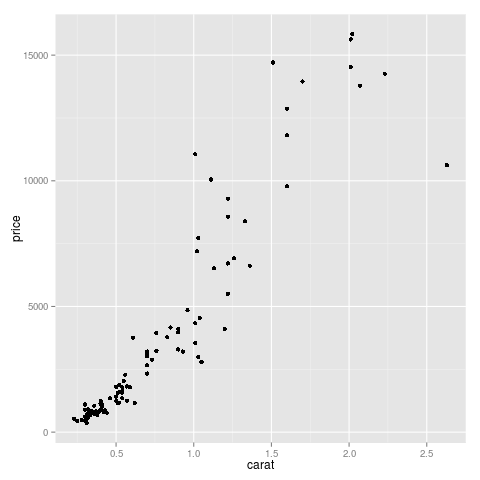
\includegraphics[width=.9\linewidth]{diamonds.png}

This opens up many opportunities for doing interesting things with R within your Org-mode documents!
\section*{Inserting \LaTeX{} output}
\label{sec-6}

We have just seen how to include graphical output in our Org-mode buffer. We can also do something similar with \LaTeX{} output generated by R. Of course, this requires at least a working \LaTeX{} installation. You will also need to install the dvipng program (\texttt{dvipng} package in Ubuntu, for instance). See the System Requirements section for other prerequisites.

\subsection*{A simple example}
\label{sec-6-1}

Let's work on a very simple example, displaying a \LaTeX{} description in our Org-mode buffer, using the official \LaTeX{} logo. We will use R to generate the code that will display the official logo. There's obviously no reason to do this except for demonstration purposes. 

First we must define an R source block that generates some \LaTeX{} code that displays the logo. That's fairly straightforward. Notice we have given the source code block a name, so that we can call it later. We use the \texttt{\#+name} syntax to do this. Note that you \textbf{don't} have to run the following code block, it will be run automatically by the next one.

\label{R-latex}
\begin{verbatim}
  latexlogo <- function() {
      "\\LaTeX"
  }
  
  latexlogo()
\end{verbatim}

Next, we define a new source block using the \texttt{latex} language, instead of \texttt{R}, as we have been using. If we use a \texttt{:file} argument with a \LaTeX{} source code block, Org-mode will generate a file of the resulting DVI file that \LaTeX{} produces, and display it. This is just like generating graphical output from R using a \texttt{:file} argument, so there is nothing new there.

However, note we have a new argument, \texttt{:noweb}. What does that mean? In short, it let's us use syntax like \texttt{<<CodeBlock()>>} to insert the results of running a code block named \texttt{CodeBlock} into another source code block. So, in our example, we're running the \texttt{R-latex} code block defined above, and inserting the results, which need to be valid \LaTeX{} code, into our \texttt{latex} code block. For this example, we of course didn't need to write an R function to generate such simple \LaTeX{} output, but it can be much more complicated, as our next example shows. In short, our R code block is helping to write the \LaTeX{} code block for us.

Noweb was not invented for Org-mode, it's been around for a while, and is used in Sweave, for example. See \href{http://en.wikipedia.org/wiki/Noweb}{its Wikipedia page}. The \texttt{:noweb} argument is set to 'no' be default, because the \texttt{<<X>>} syntax is actually valid in some languages that Org-mode supports.

Run the following code block. The \texttt{R-latex} R code block will be run, generating the string \texttt{\textbackslash{}LaTeX}, which is then substituted into this \LaTeX{} code block, and then turned into the \LaTeX{} logo by the latex program. Don't worry about the complicated header arguments, those will be explained in more detail in the next section. 

[[file:latex-logo.png]]
\subsection*{A more complicated example, exporting \LaTeX{} in buffer, to HTML, and to PDF}
\label{sec-6-2}

Now let's try something a little more complex, using an R function that generates a full \LaTeX{} table. This particular example depends on having the R package Hmisc installed. If you don't have it installed, start up R and then do: \texttt{> install.packages("Hmisc")}

What follows is an R source block that generates some \LaTeX{} code representing a table.  We want to be able to insert a \texttt{png} image of the table in the buffer when run with \texttt{C-c C-c}, using the colors of our current Emacs buffer.

A few sections from now, I'll touch on the exporting features of Org-mode.  Org can generate HTML and PDF versions of documents like this one.

Back to our example, for HTML export, we also want to generate a \texttt{png}. However, we want the background to be transparent, not whatever color our Emacs buffer happened to be.

For \LaTeX{} output, we don't need a \texttt{png} file at all, we would of course prefer to simply insert the auto-generated \LaTeX{} code in the exported \LaTeX{} document, and then compile to PDF. 

The following should accomplish all three goals.  

We tell the R code block to output latex code using the syntax \texttt{:results output latex}.  Also, only export the results.  If we export both, then the \LaTeX{} results would get exported twice when we export to PDF, once from each code block.  It would actually be exported twice when we export to HTML, but in that case, since the results are wrapped in \texttt{\#+BEGIN\_LATEX/\#+END\_LATEX} lines, and are therefore not included in the HTML export.

In the \LaTeX{} code block, a file will be generated for in-buffer evaluation and HTML export, but we don't want it produced for \LaTeX{} export, otherwise the image \emph{and} the actual table will be included in the PDF.  

The final \texttt{:buffer} argument controls the color selection through the \texttt{org-format-latex-options} variable. Essentially, if \texttt{:buffer} is set to 'yes', your Emacs buffer colors will be used as arguments to the \texttt{dvipng} program used to produce the image, assuming you don't change that values of the elements to something other than 'default' in \texttt{org-format-latex-options}. If \texttt{:buffer} is 'no', then the \texttt{html*} elements of that variable will be used.

 % latex.default(cstats, title = title, caption = caption, rowlabel = rowlabel,      col.just = col.just, numeric.dollar = FALSE, insert.bottom = legend,      rowname = lab, dcolumn = dcolumn, extracolheads = extracolheads,      extracolsize = Nsize, ...) 
%
\begin{table}[!htbp]
\caption{Descriptive Statistics by Treatment\label{summary}} 
\begin{center}
\begin{tabular}{lcccc}
\hline\hline
\multicolumn{1}{l}{}&\multicolumn{1}{c}{Active}&\multicolumn{1}{c}{Placebo}&\multicolumn{1}{c}{Combined}&\multicolumn{1}{c}{Test Statistic}\tabularnewline
&\multicolumn{1}{c}{{\scriptsize $N=57$}}&\multicolumn{1}{c}{{\scriptsize $N=43$}}&\multicolumn{1}{c}{{\scriptsize $N=100$}}&\tabularnewline
\hline
Age~at~randomization&{\scriptsize  9.52~}{10.03 }{\scriptsize 10.56} &{\scriptsize  9.51~}{10.27 }{\scriptsize 10.75} &{\scriptsize  9.51~}{10.11 }{\scriptsize 10.69} &$ F_{1,98}=0.35 ,~ P=0.554 ^{1} $\tabularnewline
Gender&&&&$ \chi^{2}_{1}=0.08 ,~ P=0.784 ^{2} $\tabularnewline
~~~~Female&37\%~{\scriptsize~$\frac{21}{~57}$}&40\%~{\scriptsize~$\frac{17}{~43}$}&38\%~{\scriptsize~$\frac{38}{100}$}&\tabularnewline
~~~~Male&63\%~{\scriptsize~$\frac{36}{~57}$}&60\%~{\scriptsize~$\frac{26}{~43}$}&62\%~{\scriptsize~$\frac{62}{100}$}&\tabularnewline
\hline
\end{tabular}
\end{center}
\noindent {\scriptsize $a$\ }{$b$\ }{\scriptsize $c$\ } represent the lower quartile $a$, the median $b$, and the upper quartile $c$\ for continuous variables.\\\indent Tests used:\\\textsuperscript{\normalfont 1}Wilcoxon test; \textsuperscript{\normalfont 2}Pearson test\end{table}

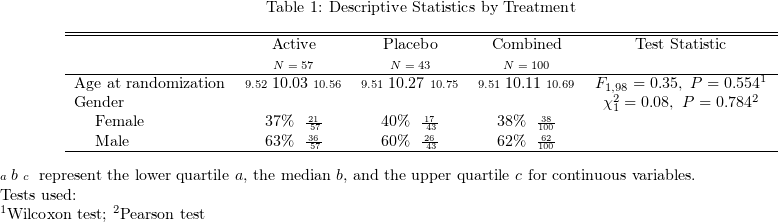
\includegraphics[width=.9\linewidth]{hmisc.png}
\section*{Putting it all together, a notebook interface to R}
\label{sec-7}

Combining the techniques shown above: submitting code blocks, capturing output for further manipulation, and inserting graphical and tabular material, we essentially have a basic notebook-style interface for R.

This is potentially useful for countless tasks such as: a laboratory notebook, time series analysis of diet/exercise habits, tracking your favorite baseball team over the course of a season, or any reporting task you can think of. Since Org-mode is a general-purpose authoring tool, with very strong exporting capabilities, almost anything is possible.

For instance, some people use Org-mode to generate HTML for blogs that they run. Several posters to the Org-mode mailing list have mentioned writing their entire graduate theses in Org-mode, and even books.

This workflow serves as an alternative to the excellent \href{http://www.stat.uni-muenchen.de/~leisch/Sweave/}{Sweave} package that cuts out the need for learning \LaTeX{} to produce high-quality documents. Org-mode is doing all the exporting for you, including \LaTeX{} if you'd like. Getting \LaTeX{} and HTML output essentially "for free" should not be underestimated!

On some level, all these activities assume that you are a comfortable Org-mode user, and that you will be writing code, conducting analyses, and possibly exporting results through the familiar Emacs and Org-mode user interface. Through the exporting functionality, Org-mode offers many useful and easy-to-use options to share \emph{results} of your efforts with others, but what about the code itself? 

Most people you have to share code with aren't going to want an Org-mode file full of source code!
\section*{Tangling code}
\label{sec-8}

With many projects, you will have to share \emph{code} with other programmers, who are most likely not going to be programming in Org-mode. Therefore, sharing an Org-mode file full of code is not an option.

Or, consider development of an R package. The package building process obviously operates on \texttt{.R} files, each full of R functions. However, that's not what we have in a document like this one.

It is in situations like these where \emph{tangling} can be used. 

The process of tangling an Org-mode document essentially extracts the code contained in Org-mode source code blocks, and places it in a file of the appropriate type. How do we do this? We use the \texttt{:tangle} source code block header argument to direct Org-mode what to do. Then, we call the tangle function on the file to extract the source code!

Read on to learn how to perform each of these steps. 

\subsection*{Instructing Org-mode how to tangle with header arguments}
\label{sec-8-1}
Let's take a look at a few examples. Each example contains an R comment, so that you can see in the resulting \texttt{.R} file where it came from.

This first example will not extract any code from the source block. It is the default behavior. 

\begin{verbatim}
# tangle was not specified
x <- 1:10
print(x)
\end{verbatim}

This will place the code in source code block in \texttt{Org-mode-R-tutorial.R}, since we don't specify a filename for the \texttt{.R} file.

\begin{verbatim}
# tangle was specified, but no file given
x <- 1:10
print(x)
\end{verbatim}

This will place the tangled code in \texttt{Rcode.R}, since we specify that name. 

\begin{verbatim}
# tangle was specified, and a file name given (Rcode.R)
x <- 1:10
print(x)
\end{verbatim}

Note that we will have multiple source code blocks in an Org-mode file, and they might have different types. For example, we might have R and Python code in the same document, but different source blocks. 

This is no problem, as the tangling mechanism will generate appropriate files of each type, containing only the code of that type.

Finally, you can specify the \texttt{:tangle} argument as a buffer-wide setting, so that you don't have to specify it for every source code block.

This opens up exciting possibilities like having a \textbf{single} Org-mode file that includes:
\begin{itemize}
\item all code for an R package
\item all documentation for the package
\item unit tests for the package
\item material to generate slides for presentations, through \texttt{org-beamer}
\item notes taken during package development
\item links to emails with bug reports, feature requests, etc.
\item a Makefile to build the package and documentation
\end{itemize}
\subsection*{Tangling the document}
\label{sec-8-2}

Now that we have seen how to instruct Org-mode how to produce source code files from our Org-mode document, how do we actually tangle the document?

We simply have to call the \texttt{org-babel-tangle} function, bound by default to \texttt{C-c C-v C-t}. 

Org-mode confirms in the minibuffer how many code blocks have been tangled, and inspecting the file system should show that your source code files have been created. There exists a hook function that will run any post-processing programs you have defined, for example, a compiler, \texttt{R CMD build}, or running \texttt{make} with a Makefile, possibly itself generated from the Org-mode document!
\section*{Exporting documents containing code and results}
\label{sec-9}

Org-mode provides a rich set of functions and customizations for exporting documents into more human-readable forms, and for users who are not Emacs or Org-mode users. The most common methods are generating PDF documents through \LaTeX{}, and HTML output. Source code will be syntax highlighted, in HTML.  There are various options for PDF, including using the listings package.

With Org-mode source blocks, you can choose to export the source code, the results of evaluating the source code, neither, or both. The \texttt{:exports} header argument controls this. See the \href{http://orgmode.org/manual/Exporting-code-blocks.html#Exporting-code-blocks}{documentation} for further examples. 

As an example, type \texttt{C-c C-e h o} to see an HTML version of this document.

Some fairly sophisticated processes, including complete report generation using R graphics and tables, can be achieved through this facility.

Using Org-mode in this manner is essentially an alternative to Sweave, with the advantages of:
\begin{itemize}
\item do not need to learn \LaTeX{} or other markup language
\item any future Org-mode export engines will be available to you
\item writing code in Org-mode gives you access to a hyper-commenting system, with features such as TODO items, in-document linking, tags, and code folding.
\end{itemize}

If you're an advanced \LaTeX{} user, you probably don't view point 1 above as an advantage. :) 

Whether or not you use all the features that Org-mode provides, you can use the system for literate programming and reproducible research, on projects large and small.
\section*{Where to go from here?}
\label{sec-10}

We have seen how to submit R code for evaluation in Org-mode. There are many good reasons to do this, including tying results to source code, code folding, exporting of code and results into many common formats, improving documentation, and the innumerable features that Org-mode provides, and will continue to provide in the future. 

As with all new processes, it can be a challenge to start working with source code this way.  For what to do next, try looking at the \href{http://orgmode.org/worg/org-contrib/babel/uses.php}{results} of some of those who use Org-mode to accomplish interesting things. You can look at current documentation for R support \href{http://orgmode.org/worg/org-contrib/babel/languages/ob-doc-R.html}{here}.

For an exercise in using Org-mode with source code, you can write your Emacs initialization file in Org-mode! These \href{http://orgmode.org/worg/org-contrib/babel/intro.php#sec-8_2_1}{instructions} are slightly out of date, but they give you a general idea of how to proceed. Essentially, your master Emacs init file will simply tangle an Org-mode file full Emacs lisp code blocks, and then load the resulting file.

In short, there are many possibilities using these techniques! In many ways, this tutorial only scratches the surface of Org-mode's capabilities. As always, the \href{http://orgmode.org/manual/index.html#Top}{official manual} will be the source of the most up-to-date information and features of this great tool.
% Generated by Org mode 7.9.3e in Emacs 24.3.50.1.
\end{document}